% !TEX program = pdflatex
\documentclass[11pt,a4paper]{article}

\usepackage[utf8]{inputenc}
\usepackage[T1]{fontenc}
\usepackage{lmodern}
\usepackage{geometry}
\geometry{margin=1in}
\usepackage{amsmath,amssymb}
\usepackage{siunitx}
\usepackage{graphicx}
\usepackage[font=small,labelfont=bf,labelsep=endash]{caption}
\usepackage{booktabs}
\usepackage{physics}
\usepackage{hyperref}
\usepackage{float}
\hypersetup{colorlinks=true,linkcolor=blue,citecolor=blue,urlcolor=blue}


\title{Design Methodology for a Dual-Jet Hovering Disc with Concentric Air Curtains:\\
Model, Non-Dimensionalization, and Physical Assumptions}
\author{ }
\date{ }

\begin{document}
\maketitle

\begin{abstract}
This paper presents a design-oriented physical model for a hovering disc sustained by two concentric air jets: 
an outer annular jet that forms an aerodynamic curtain to confine the inner flow and an inner jet that maintains the central cushion pressure.
The analysis uses a low-Mach compressible, axisymmetric core model with an anisotropic Stokes--Darcy closure to approximate the pressure and velocity fields in the cushion region.
A detailed discussion of the model's assumptions and their physical validity is provided, along with a complete nomenclature of symbols used throughout the work.
\end{abstract}

\section{Geometry and Notation}
The geometry follows Fig.~\ref{fig:geometry}, defining the coordinate system and characteristic dimensions:
\begin{itemize}
  \item $R_{\mathrm{tot}}$ -- total radius of the disc.
  \item $h$ -- hovering height from the ground.
  \item $w$ -- width of the peripheral leakage ring; $R^{-}=R_{\mathrm{tot}}-w$ is its inner radius.
  \item $b$ -- thickness of the outer annular jet slot.
  \item $h_{\mathrm{eff}}$ -- effective sealing height (characteristic of curtain recirculation).
  \item $p_0$ -- ambient pressure; $p_c=W/(\pi R_{\mathrm{tot}}^2)$ -- cushion pressure supporting the load $W$.
  \item $U_{\mathrm{out}}$, $\rho_j$ -- speed and density of the outer jet.
  \item $\mu$ -- dynamic viscosity; $R_g$ -- specific gas constant for air.
  \item $\dot{m}_{\mathrm{in}}$ -- air mass flow entering internal region.
  \item $\dot{m}_{\mathrm{out}}$ -- air mass flow of outer region.
  \item $\dot{m}_{\mathrm{loss}}$ -- air mass flow exiting internal region.
\end{itemize}

\begin{figure}[t]
  \centering
  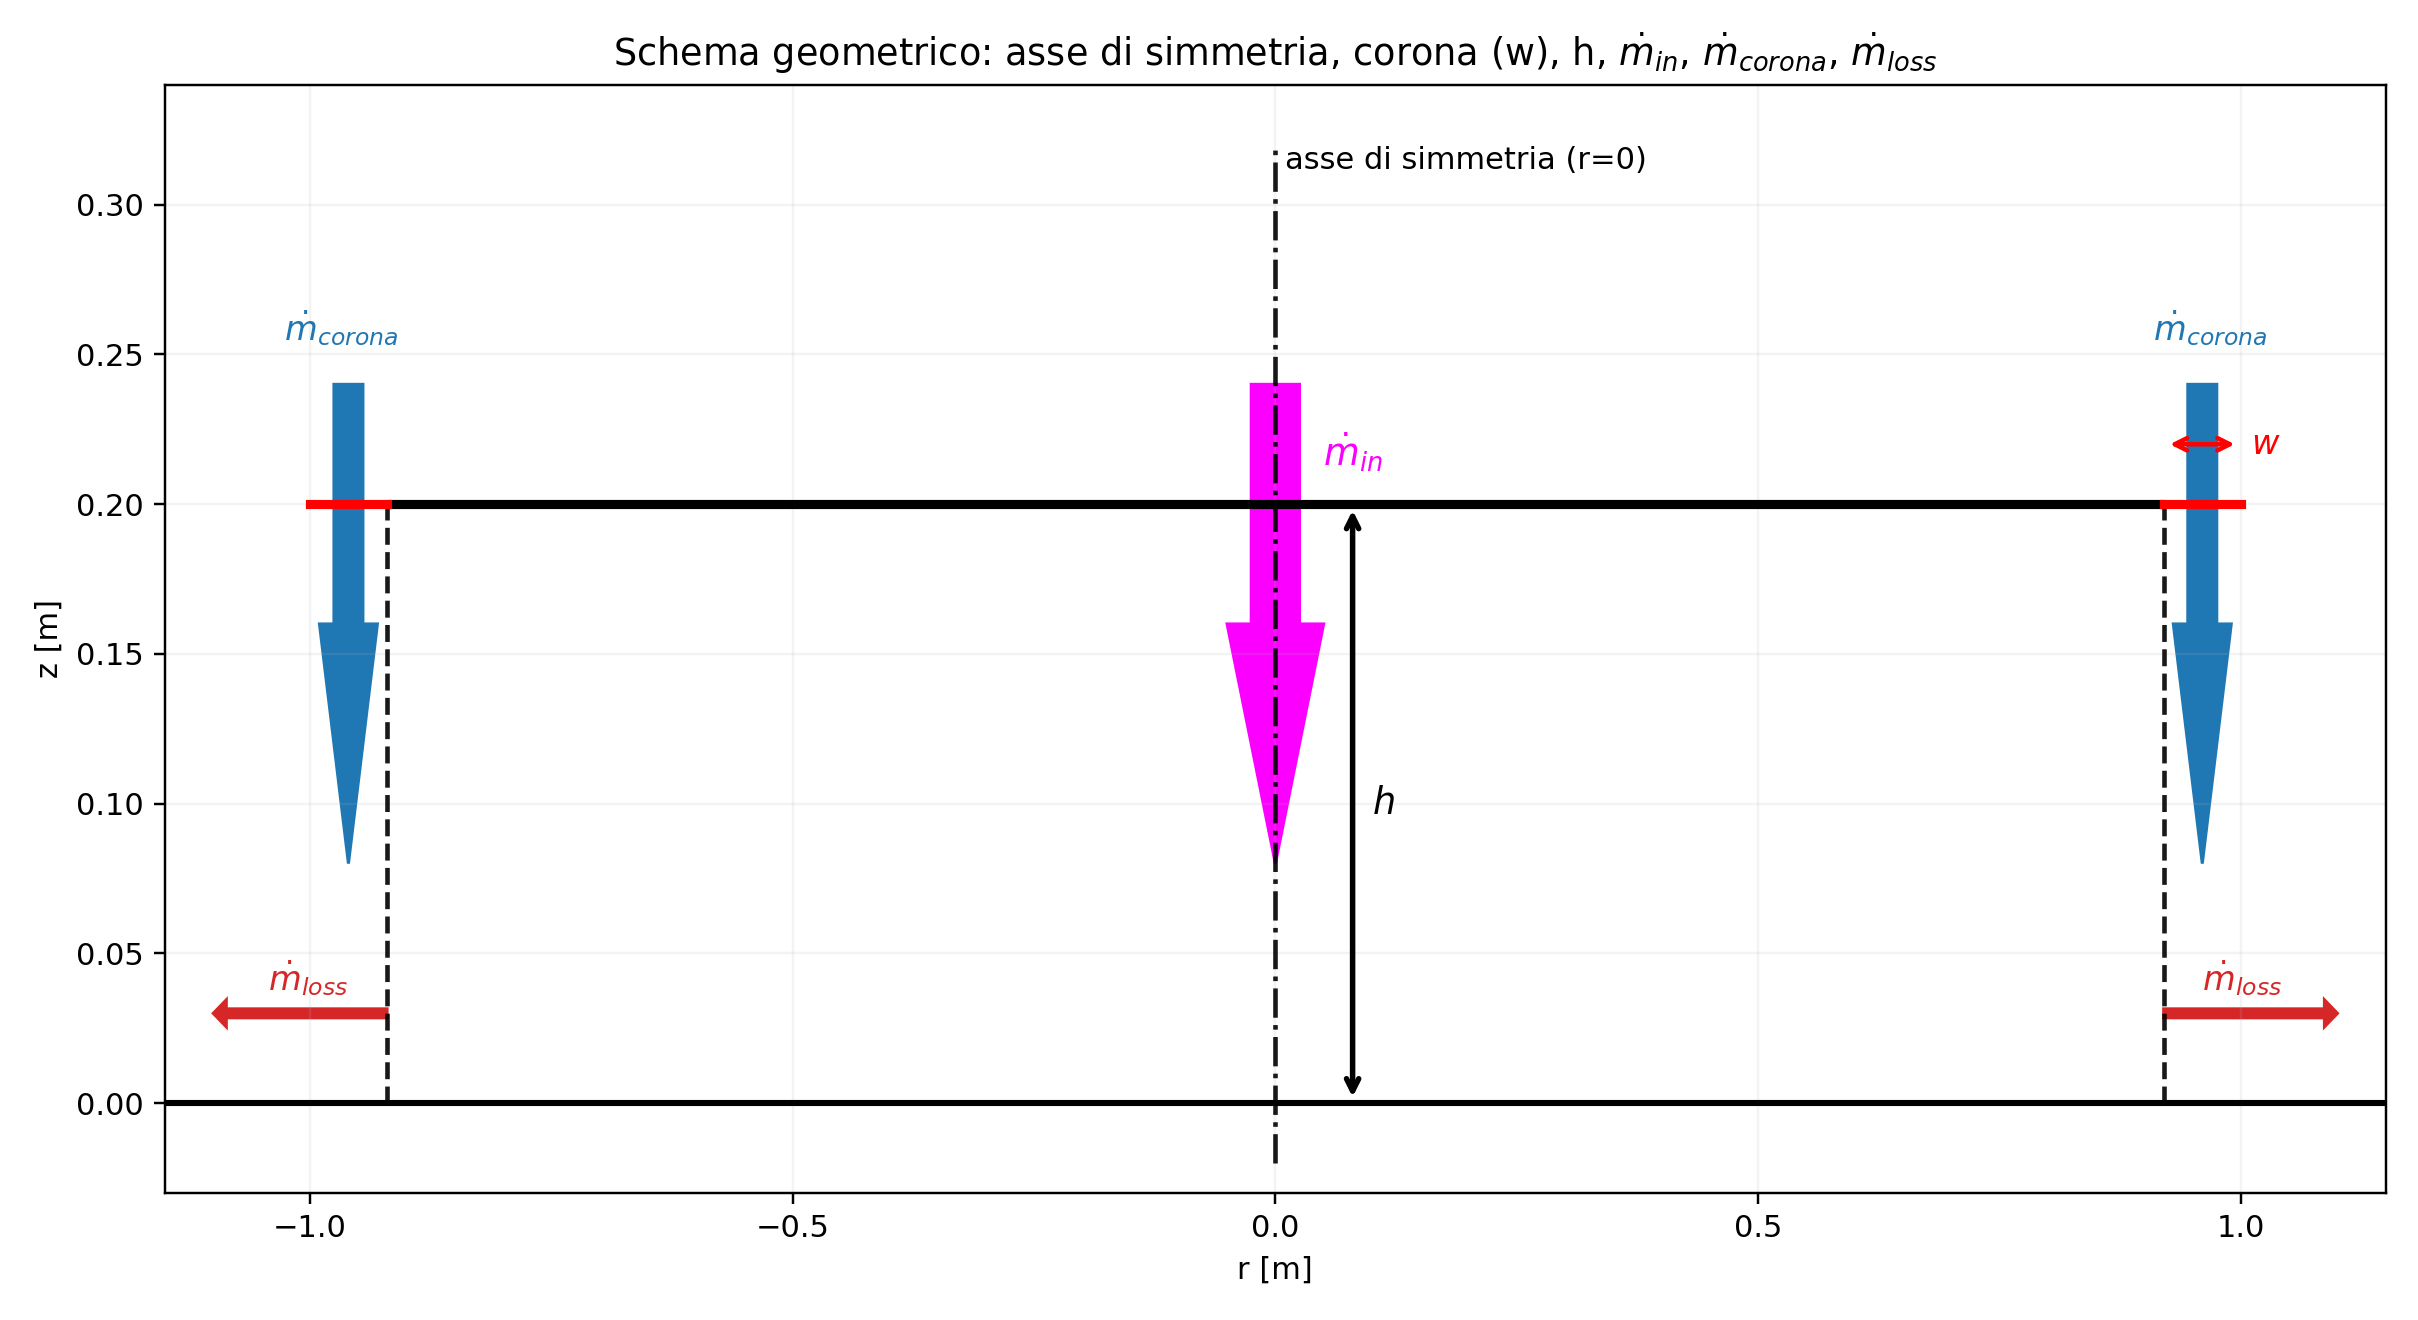
\includegraphics[width=0.95\linewidth]{../figs/schema_geometry.png}
  \caption{Schematic of the hovering disc with two concentric jets: the outer annular curtain and the central make-up flow.}
  \label{fig:geometry}
\end{figure}

\section{Model Overview}
The cushion region ($0\le r\le R^{-},\ 0\le z\le h$) is filled with air at variable pressure, temperature, and density. 
The mean flow satisfies an anisotropic Stokes--Darcy closure:
\begin{equation}
  u = -\frac{\kappa_r}{\mu}\,\partial_r p,\qquad
  w = -\frac{\kappa_z}{\mu}\,\partial_z p,
\end{equation}
with permeability coefficients $\kappa_r=\alpha_r h^2$ and $\kappa_z=\alpha_z h^2$, where $\alpha_r$ and $\alpha_z$ are empirical dimensionless parameters encoding the overall resistance of the confined air layer.

The continuity and state relations read
\begin{equation}
  \frac{1}{r}\,\partial_r\!\left(r\rho u\right)+\partial_z(\rho w)=0,\qquad
  p=\rho R_g T.
\end{equation}
Elimination of $u,w$ gives the pressure formulation:
\begin{equation}
  \frac{1}{r}\partial_r(r\rho\kappa_r\partial_r p)+\partial_z(\rho\kappa_z\partial_z p)=0.
\end{equation}

\section{Validity of Modeling Assumptions}
\subsection{Low-Mach Compressibility}
The jets have typical velocities $U_{\mathrm{out}}\approx30$--$60\,$m/s, leading to a Mach number $Ma=U/a\approx0.1$--$0.2$ with $a\simeq343\,$m/s. 
This regime justifies a \emph{low-Mach} formulation: the flow is compressible enough to exhibit pressure- and temperature-dependent density, but acoustic effects remain negligible. 
Hence, the ideal-gas relation $p=\rho R_g T$ is retained, while the flow is assumed quasi-static in time.

\subsection{Thermal Uniformity and Energy Exchange}
Although the confined air experiences some compression heating, the characteristic time scales of thermal diffusion and convective mixing by the curtain are short compared to global unsteadiness. 
The first-order model therefore assumes a uniform temperature $T=T_\infty$, with the understanding that future extensions may include the steady energy balance to recover small deviations of $T(r,z)$.

\subsection{Stokes--Darcy Closure}
The Stokes--Darcy model does not imply a porous medium in the literal sense. 
Instead, it approximates the momentum balance of a low-Reynolds, highly dissipative, confined flow.
At low $Re=\rho U h/\mu$, the Stokes equations reduce to a linear proportionality between pressure gradient and velocity.
Replacing $\nabla^2\mathbf{u}\sim \mathbf{u}/L^2$ with an effective geometric length $L\sim h$ yields
\begin{equation}
  \mathbf{u}\approx-\frac{h^2}{\mu}\nabla p,
\end{equation}
which is mathematically equivalent to Darcy’s law with an effective permeability $\kappa\sim h^2$.
The anisotropic form used here,
\begin{equation}
  \kappa_r=\alpha_r h^2,\qquad \kappa_z=\alpha_z h^2,
\end{equation}
accounts for different confinement levels in the radial and vertical directions.

\paragraph{Validity range.} 
This closure is valid provided that:
\begin{itemize}
  \item the Reynolds number in the cushion $Re_c=\rho U_c h/\mu \ll 1$;
  \item pressure variations are slow and inertia negligible;
  \item the flow is quasi-steady and dominated by viscous losses and boundary friction;
  \item local turbulence and recirculation effects are absorbed into the empirical coefficients $\alpha_r,\alpha_z$.
\end{itemize}
It is particularly suited to parametric design and control studies where the detailed jet micro-structure is not resolved.

\subsection{Boundary Conditions and Curtain Coupling}
The outer slot jet issues \emph{downwards} and acts as an \emph{air curtain} that
limits radial leakage from the cushion. The pressure imposed along the rim
$r=R^{-}$ is modeled as the superposition of two physically motivated
contributions:
\begin{equation}
  p_{\mathrm{edge}}(z)
  = p_0 + \rho_j U_{\mathrm{out}}^2\,
    \big[\, C_p\, (1-\zeta)^{n} \;+\; C_s\, \zeta^{m} \,\big],
  \qquad \zeta=\frac{z}{h}.
  \label{eq:rim_pressure_composite}
\end{equation}
The first (static) term approximates the increase of static pressure associated with
jet deceleration and turning near the floor ($\zeta\!\to\!0$). The second (sealing)
term represents the \emph{barrier effectiveness} near the slot ($\zeta\!\to\!1$),
which grows with jet momentum. Typical choices are $m,n\in[1,2]$ and
$C_p,C_s=O(10^{-1}\!\!-\!1)$; in the simplest reduced form, one may merge both
effects into a single effective coefficient $C_t$,
$\Delta p = C_t \rho_j U_{\mathrm{out}}^2 b / h_{\mathrm{eff}}$.

On $z=0$ and $z=h$ we impose no-normal-flow in the reduced core model
\begin{equation}
  \partial_z p(r,0)=\partial_z p(r,h)=0,
\end{equation}
while $r=0$ enforces symmetry $\partial_r p(0,z)=0$. The inner make-up jet is not
imposed as a local BC in the core; its effect enters the \emph{global} mass balance
(see Sec.~\ref{sec:shooting}).
This expression guarantees continuity of rim pressure along $z$ and smoothly connects
the low static pressure region at the slot exit with the higher static build-up near the
floor.

\paragraph{Remark on sealing vs static pressure.}
The composite rim pressure in Eq.~\eqref{eq:rim_pressure_composite} is a
\emph{modeling device}: the $(1-\zeta)^n$ term provides a minimal representation
of static-pressure build-up as the curtain turns near the floor, while the
$\zeta^m$ term encodes the sealing effectiveness of a high-momentum jet near the slot.
This separation avoids conflating the jet’s low static pressure near the slot with
its strong \emph{barrier} effect on radial leakage.

\section{Core Model and Sealing Condition (summary)}
We adopt the anisotropic Stokes--Darcy closure for mean velocities
\begin{equation}
  u = -\frac{\kappa_r}{\mu}\,\partial_r p,\qquad
  w = -\frac{\kappa_z}{\mu}\,\partial_z p,\qquad
  \kappa_r=\alpha_r h^2,\ \kappa_z=\alpha_z h^2,
\end{equation}
together with compressible continuity and the ideal-gas state $p=\rho R_g T$.
The design-oriented pressure equation in the core is
\begin{equation}
  \frac{1}{r}\,\partial_r\!\big(r\,\rho\,\kappa_r\,\partial_r p\big)
  +\partial_z\!\big(\rho\,\kappa_z\,\partial_z p\big)=0,
\end{equation}
with BCs: symmetry at $r=0$; no-normal-flow at $z=0$ and $z=h$; and a rim pressure
at $r=R^{-}$ given by the composite sealing model in
Eq.~\eqref{eq:rim_pressure_composite}:
\begin{equation}
  p_{\mathrm{edge}}(z) = p_0 + \rho_j U_{\mathrm{out}}^2
  \big[ C_p(1-\zeta)^{n} + C_s \zeta^{m} \big], \qquad \zeta=z/h.
\end{equation}
Here the sealing contribution models the barrier action of the downward curtain
(rising with jet momentum near the slot), while boundaries at $z=0,h$ remain
impermeable in the reduced core. The coefficients $C_p$ and $C_s$ retain the same meaning and order of magnitude as
introduced in Sec.~\ref{sec:boundaryconditions}.



\section{Non-Dimensionalization and Plotting Conventions}
We scale
\begin{equation}
  \hat r=\frac{r}{R_{\mathrm{tot}}},\quad
  \hat z=\frac{z}{h},\quad
  \hat p=\frac{p-p_0}{p_c},\quad
  \hat T=\frac{T}{T_\infty},\quad
  \hat\rho=\frac{\rho}{\rho_\infty}=\frac{1+\Pi_p\,\hat p}{\hat T},\ \ \Pi_p=\frac{p_c}{p_0}.
\end{equation}
with boundary conditions
\begin{equation}
  \partial_{\hat r}\hat p(0,\hat z)=0,\qquad
  \partial_{\hat z}\hat p(\hat r,0)=\partial_{\hat z}\hat p(\hat r,1)=0,\qquad
  \hat p(\hat R^{-},\hat z)=
  \Pi_{\mathrm{edge}}\,
  \big[\, C_p (1-\hat z)^{n} + C_s \hat z^{m} \,\big],
\end{equation}
where $\hat R^{-}=R^{-}/R_{\mathrm{tot}}$ and
$\Pi_{\mathrm{edge}}=(p_{\mathrm{edge}}-p_0)/(\rho_j U_{\mathrm{out}}^2)$ (so that
$C_p,C_s$ are dimensionless). If one prefers a single effective term,
set $C_p=0$ and rename $C_s\to C_t$. When using the composite form, $C_t$ is omitted and replaced by $(C_p,C_s)$ as separate
dimensionless sealing coefficients.

Natural velocity scales are
\begin{equation}
  U_r^0=\frac{\kappa_r}{\mu}\,\frac{p_c}{R_{\mathrm{tot}}},\qquad
  U_z^0=\frac{\kappa_z}{\mu}\,\frac{p_c}{h},\qquad
  S=\frac{U_z^0}{U_r^0}=\frac{\alpha_z}{\alpha_r}\frac{R_{\mathrm{tot}}}{h}.
\end{equation}
The dimensionless velocities for plotting are
\begin{equation}
  \hat u=-\partial_{\hat r}\hat p,\qquad
  \hat w=-\partial_{\hat z}\hat p,\qquad
  \hat V_{\mathrm{iso}}=\sqrt{\hat u^{\,2}+S^{2}\hat w^{\,2}}.
\end{equation}

\section{Mass-Balance Closure via Shooting}
\label{sec:shooting}
The core solve provides $p(r,z)$ given the rim distribution. To enforce the lift
constraint $\overline{p}=p_c$ and recover flows and power, we adopt:
\begin{enumerate}
  \item Choose an initial curtain intensity (e.g.\ $U_{\mathrm{out}}$ or $C_t$), hence
        $\Pi_{\mathrm{edge}}$.
  \item Solve the core equation with the rim Dirichlet condition.
  \item Compute the area-mean cushion pressure over the core
  \[
    \overline{p}_{\mathrm{core}}=\frac{1}{\pi (R^-)^2}
    \int_0^{R^{-}}\!\!\int_0^h (p-p_0)\,2\pi r\,dz\,dr.
  \]
  Let $p_c^{\mathrm{core}} = p_c \left(\frac{R_{\mathrm{tot}}}{R^-}\right)^2$ denote the
  target mean over the core compatible with the original definition
  $p_c=W/(\pi R_{\mathrm{tot}}^2)$.
  \item If $\big|\overline{p}_{\mathrm{core}}-p_c^{\mathrm{core}}\big|>\varepsilon$, update
  the curtain intensity and repeat.

  \item With $\overline{p}=p_c$, estimate lateral losses $\dot m_{\mathrm{loss}}$ (thin-film
  or orifice model depending on $Re_h$) and the make-up flow
  \(
    \dot m_{\mathrm{in}}=\dot m_{\mathrm{loss}}-\beta\,\dot m_{\mathrm{out}},
  \)
  where $\beta$ will be implemented in the next code revision. The shaft power follows
  from the pressure rises in the two jet circuits.
\end{enumerate}
The shooting procedure therefore adjusts the curtain intensity until the mean cushion
pressure over the core area equals $p_c^{\mathrm{core}}$.


\section{Simulation Outputs}
The results produced from the model are shown in this section.
\begin{figure}[H]
  \centering
  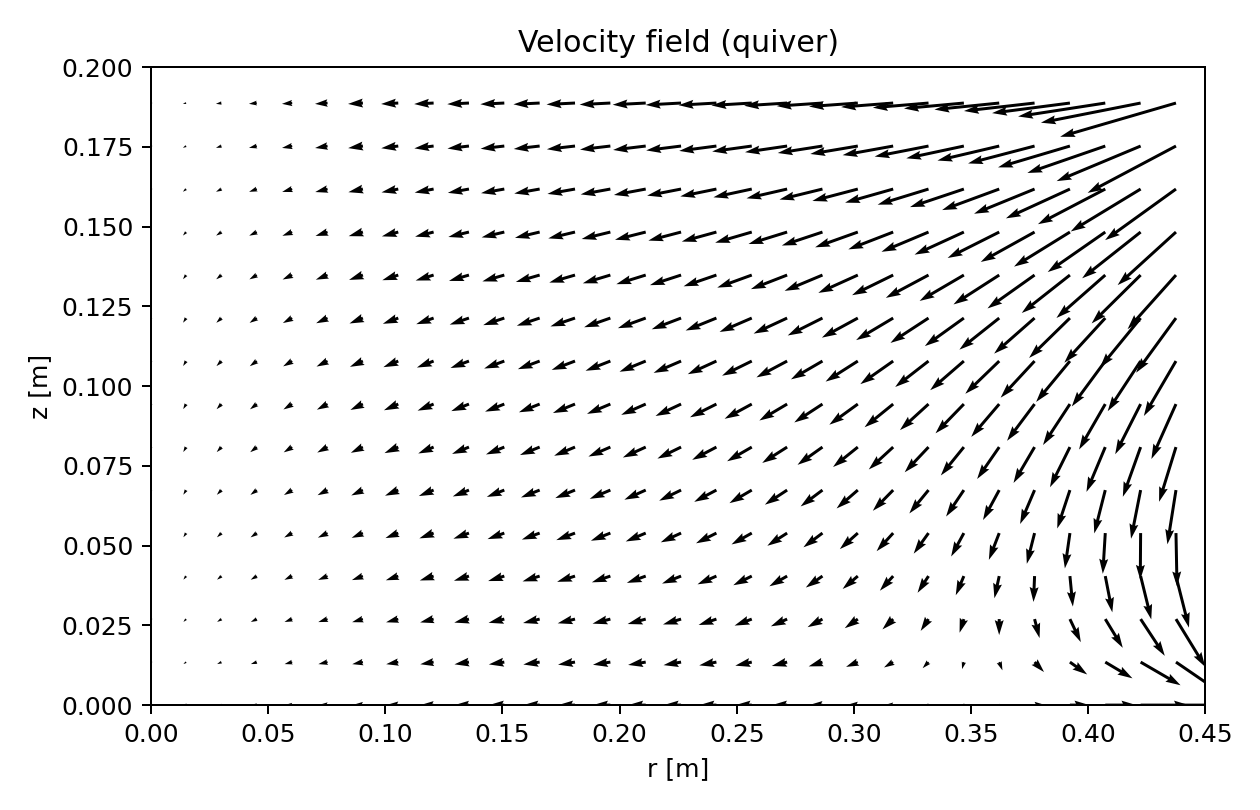
\includegraphics[width=0.95\linewidth]{../figs/quiver_velocity.png}
  \caption{Non-dimensional velocity field (quiver).
Vectors show $(\hat u,\,S\hat w)$ for isotropic visual scaling; the pattern reflects the rim-imposed sealing pressure from the downward curtain.}
  \label{fig:quiver}
\end{figure}

\begin{figure}[H]
  \centering
  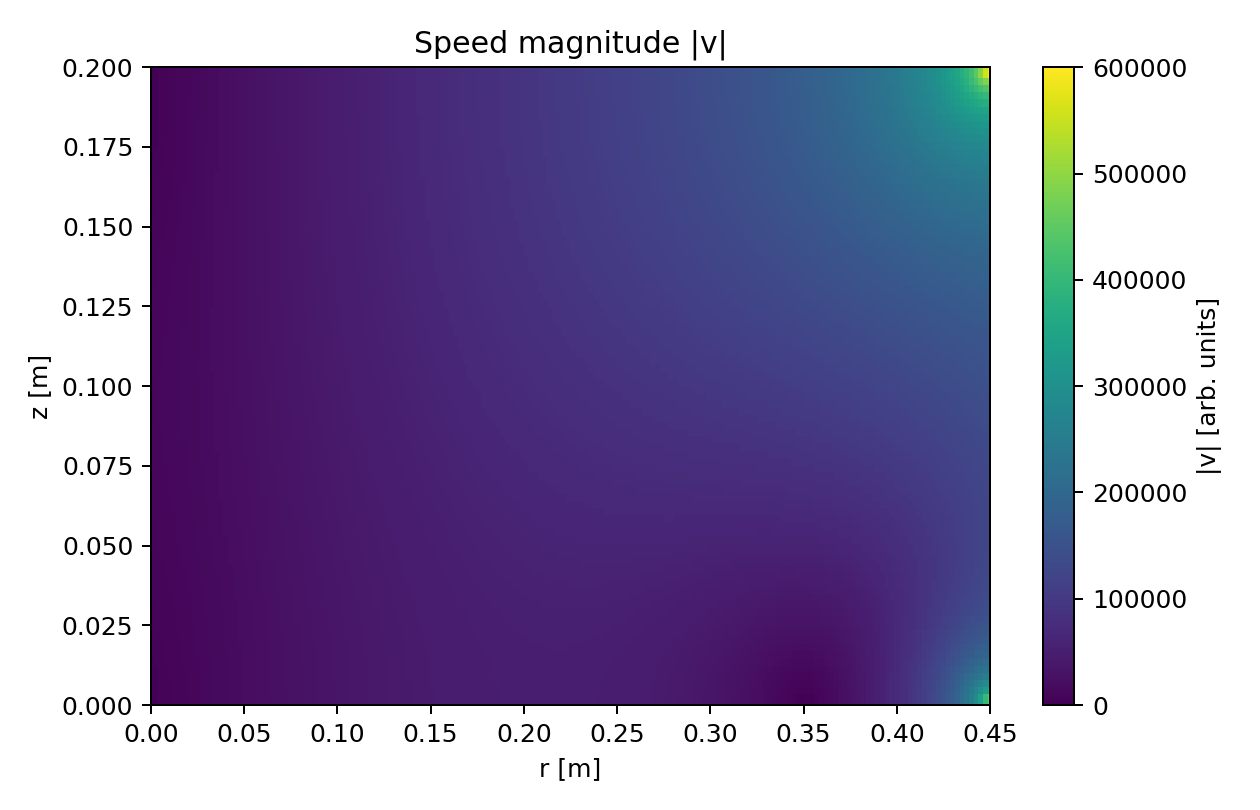
\includegraphics[width=0.95\linewidth]{../figs/cmap_speed.png}
  \caption{Colormap of the non-dimensional isotropic speed magnitude $\hat V_{\mathrm{iso}}=\sqrt{\hat u^{\,2}+S^{2}\hat w^{\,2}}$.}
  \label{fig:cmap_speed}
\end{figure}

\begin{figure}[H]
  \centering
  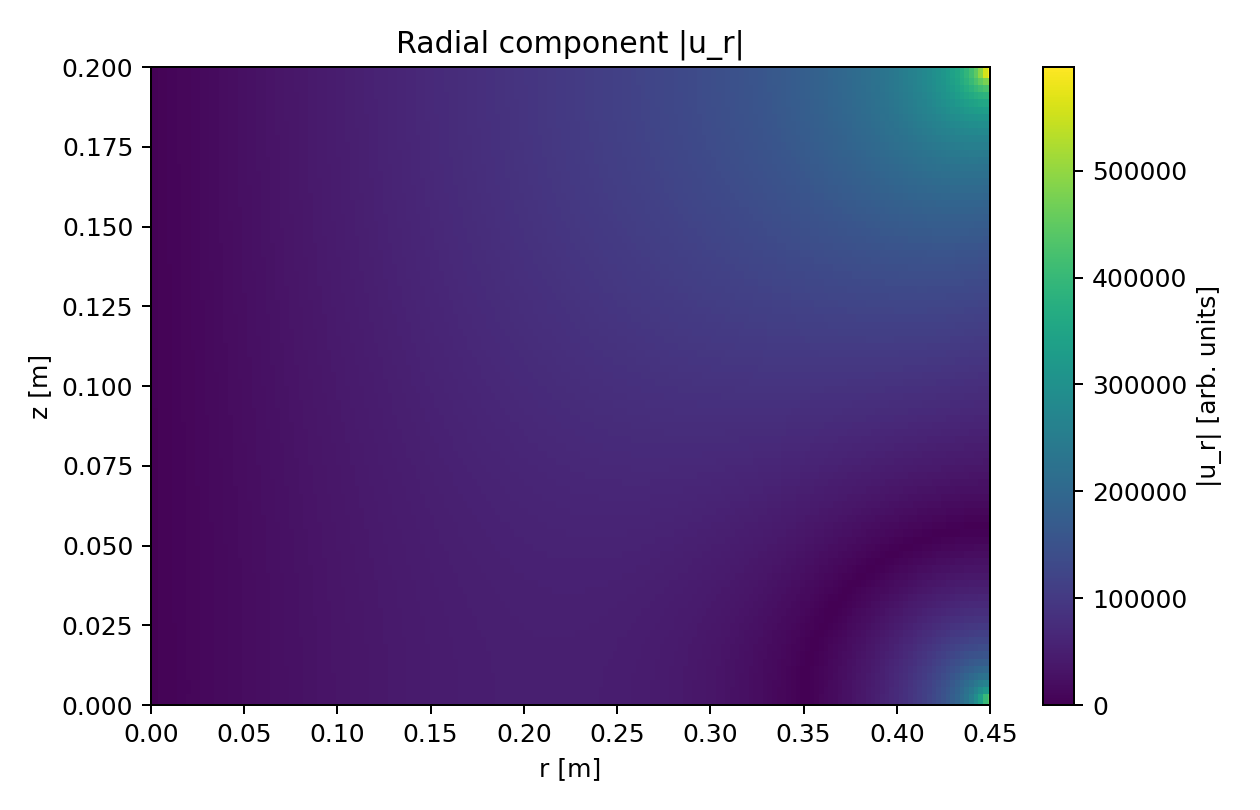
\includegraphics[width=0.95\linewidth]{../figs/cmap_ur.png}
  \caption{Colormap of the non-dimensional radial component magnitude $|\hat u|$.}
  \label{fig:cmap_ur}
\end{figure}

\begin{figure}[H]
  \centering
  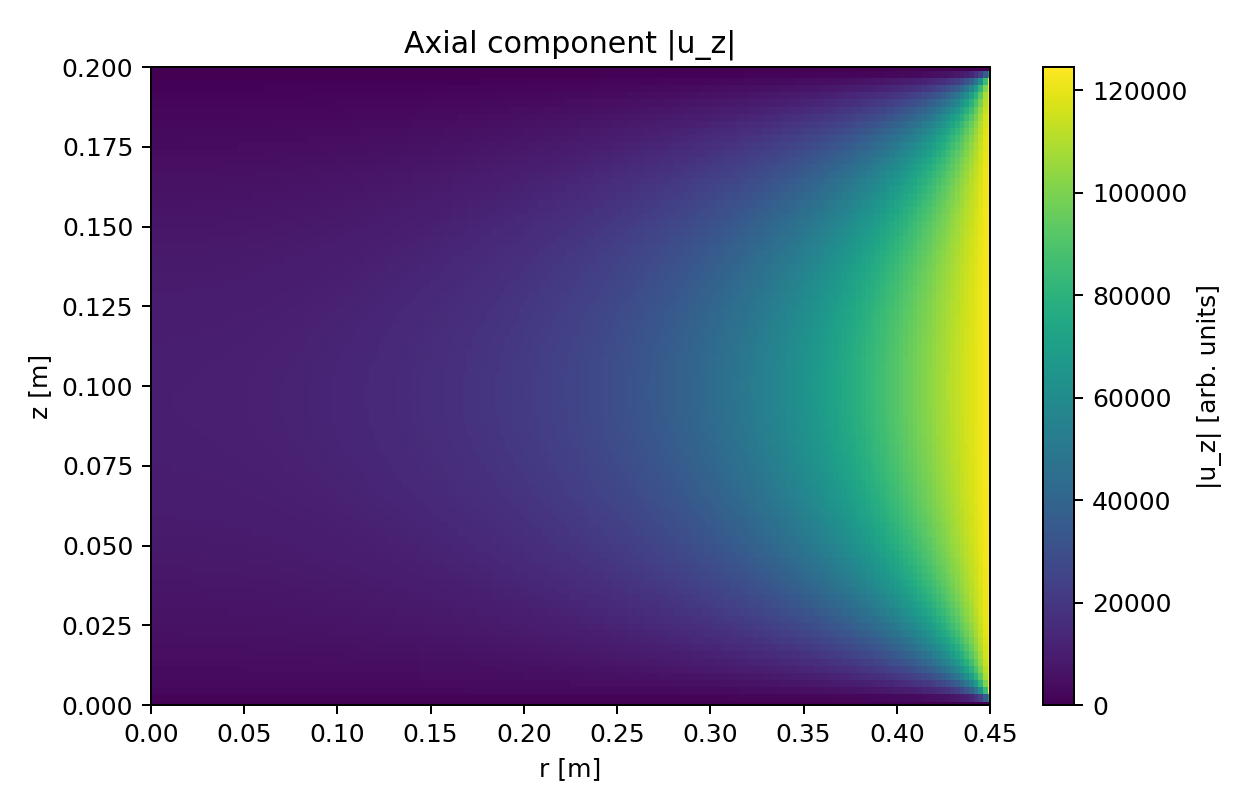
\includegraphics[width=0.95\linewidth]{../figs/cmap_uz.png}
  \caption{Colormap of the non-dimensional axial component magnitude $|\hat w|$.}
  \label{fig:cmap_uz}
\end{figure}

\begin{figure}[H]
  \centering
  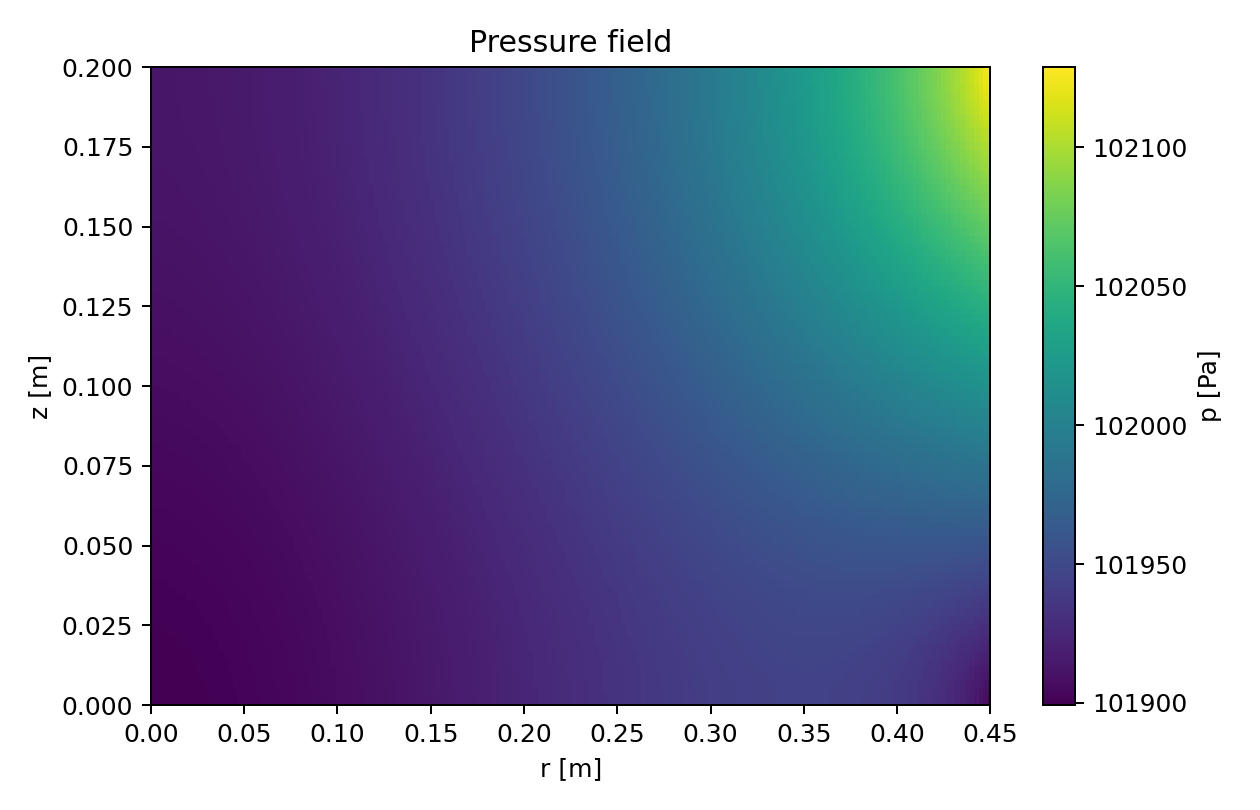
\includegraphics[width=0.95\linewidth]{../figs/cmap_pressure.png}
  \caption{Colormap of the non-dimensional pressure $\hat p$.}
  \label{fig:cmap_p}
\end{figure}

\section{Model Limitations and Planned Extensions}
The Darcy--Brinkman closure is an engineering reduction (effective permeability in a
free flow); $\alpha_r,\alpha_z$ should be calibrated against axisymmetric CFD.
The make-up jet is not imposed as a local BC in the core; it enters only via the
mass-balance closure. Thermal effects are neglected ($T=T_\infty$). The bypass parameter
$\beta$ is defined conceptually but not used yet in the code; it will be included together
with the automated shooting loop and power estimates.

\paragraph{Appendix: minimal rationale for the composite rim pressure.}
Consider a control volume hugging the rim over height $h$ and thickness $O(b)$.
A downward slot jet of density $\rho_j$ and speed $U_{\mathrm{out}}$ is deflected
into a radial wall-jet of speed $U_r(z)$ near the floor. A crude momentum balance
suggests a static build-up $\Delta p_{\mathrm{stat}}\sim \rho_j U_{\mathrm{out}}^2
\,\mathcal{O}(1)$ concentrated near $\zeta\!\to\!0$, while the resistance to
cross-flow (sealing) scales with the jet momentum flux impinging near the slot,
$\Delta p_{\mathrm{seal}}\sim \rho_j U_{\mathrm{out}}^2\,\mathcal{O}(1)$ for
$\zeta\!\to\!1$. The composite form
$\rho_j U_{\mathrm{out}}^2\,[\,C_p(1-\zeta)^n + C_s \zeta^m\,]$ is thus a
first-order surrogate capturing both effects with two tunable, dimensionless
coefficients $(C_p,C_s)$ and mild shape exponents $(m,n)$.


\section{Nomenclature}
\begin{tabular}{@{}ll@{}}
\toprule
Symbol & Description \\ \midrule
$R_{\mathrm{tot}}$ & Total radius of the disc \\
$R^{-}$ & Inner radius of the leakage ring ($R^{-}=R_{\mathrm{tot}}-w$) \\
$w$ & Width of peripheral leakage region \\
$h$ & Hovering height (disc--ground gap) \\
$h_{\mathrm{eff}}$ & Effective sealing height at rim \\
$b$ & Slot thickness of the curtain jet \\
$U_{\mathrm{out}}$ & Outer jet velocity \\
$\rho_j$ & Density of outer jet \\
$\rho$ & Density in the core region \\
$p,p_0,p_c$ & Local, ambient, and cushion pressures \\
$T,T_\infty$ & Local and ambient temperatures \\
$\mu$ & Dynamic viscosity of air \\
$R_g$ & Specific gas constant of air \\
$W$ & Payload supported by cushion \\
$\kappa_r,\kappa_z$ & Effective permeabilities (radial/axial) \\
$\alpha_r,\alpha_z$ & Dimensionless permeability coefficients \\
$u,w$ & Velocity components (radial, vertical) \\
$\Phi(z)$ & Dimensionless rim-pressure distribution \\
$C_t$ & Curtain transfer coefficient \\
$\Delta p$ & Rim pressure increment \\
$\Pi_{\mathrm{edge}}$ & Dimensionless rim pressure amplitude \\
$\mathcal{A}$ & Permeability anisotropy parameter \\
$\hat r,\hat z,\hat p$ & Dimensionless coordinates and pressure \\
$\hat u,\hat w$ & Dimensionless velocity components \\
$S$ & Velocity anisotropy ratio $S=(\alpha_z/\alpha_r)(R_{\mathrm{tot}}/h)$ \\ \bottomrule
$C_p$ & static-pressure coefficient for rim build-up (order $10^{-1}$)\\
$C_s$ & sealing-effectiveness coefficient for high-momentum curtain (order $1$)\\
$m,n$ & shape exponents for sealing and static contributions, respectively\\
\end{tabular}

\end{document}
